\documentclass[a4paper, 10pt]{article}
\usepackage[utf8]{inputenc}
\usepackage{amssymb}
\usepackage{amsmath}
\usepackage{graphicx}

\title{Object Recognition by Physical Properties Detection using Fault Reconstruction Techniques}
\author{Marco Negrete and Jesús Savage}
\date{RCF-MathWorks Fund - Call 2020\\Technical Report}

\begin{document}
\maketitle

\section{Introduction}
\subsection{Motivation}
Consider the following serving-drinks-test scenario: a robot is asked to bring beverages and to do so, the robot performs the following common steps: it navigates to the bar, recognizes the beverages (usually cans or tetra packs), calculate some sort of inverse kinematics, moves its manipulator, grasps the object and returns to the user's location. This is a common situation in @Home tasks, nevertheless, what happens if there are empty cans or tetra packs in the bar? As it is commonly implemented in @Home league, robots are unable to distinguish between empty and full cans, since they commonly rely only in visual recognition of the beverage containers (see, for example, description papers of last edition winner teams \cite{tdp2019Eindhoven, tdp2019Homer, tdp2019UTS}).
\subsection{Objectives and goals}
The project we propose consist in applying model based fault reconstruction techniques \cite{ding2013model} to estimate the weight of the object being carried by the robot. If we consider the manipulator without load in the final effector as the nominal system, and the weight of the object as an external perturbation causing a faulty behavior, we can apply MBFRA to estimate such perturbation, i.e., to estimate object's weight. There are several approaches for MBFR. Residual generation is a common technique where an observer is designed to be sensitive to fault signals. On the other hand, Sliding Mode Observers (SMO) are dynamic estimators designed to be robust against fault signals \cite{shtessel2014sliding}. SMOs also provide the ability to reconstruct the fault signal by filtering the so called output error injection term \cite{alwi2011fault}.

\section{Background}
\subsection{Sliding Mode Observers}
Sliding mode observers have the properties of ...

\subsection{Robot Justina's manipulator}
Justina is a domestic service robot built at the Biorobotics Laboratory of the National Autonomous University of Mexico and developed under the ViRBot architecture \cite{savage2008virbot}. This robot and its predecessors have been participating in the Robocup@Home league \cite{wachsmuth2015robocup} since 2006 performing several tasks such as cleaning a table, serving drinks and several other tasks that humans ask for. 

Among other actuators, Justina has two 7-DOF manipulators built with Dynamixel servomotors. Such servomotors allow the user to control them in several forms: by setting a goal position, setting a goal movement speed or setting a desired current which will produce a torque. This latter option is used in this project. Also, these motors provide position sensing with a resolution of less than a tenth of degree. Figure \ref{fig:Justina} shows robot Justina and its sensors and actuators. 
\begin{figure}
  \centering
  \includegraphics[width=0.6\textwidth]{Figures/Justina.png}
  \caption{The domestic service robot Justina.}
  \label{fig:Justina}
\end{figure}

To describe the kinematic chain and some physical properties of the manipulator, we use an URDF file. This file was used as a starting point for modeling and simulation purposes, as described in section SADFSAF. Figure \ref{fig:left_arm} shows the left arm of robot Justina as represented in the URDF.
\begin{figure}
  \centering
  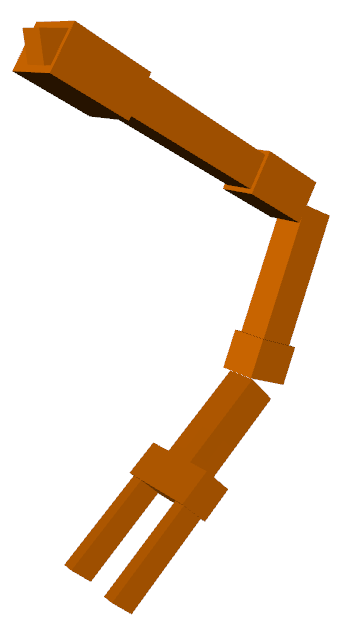
\includegraphics[width=0.4\textwidth]{Figures/left_arm.png}
  \caption{The left arm of robot Justina.}
  \label{fig:left_arm}
\end{figure}


\section{Mass estimation with Sliding Mode Observers}
\subsection{Dynamic Model}
  From the Langrangian of the manipulator, a dynamic model of the following form can be obtained:
  \begin{equation}
    M(q)\ddot{q} + C(q, \dot{q})\dot{q} + B\dot{q} + G(q) + \Delta(q,\dot{q}, u) = u
    \label{eq:lagrangian}
  \end{equation}
  where $q\in \mathbb{R}^7$ are the joint angles, $M(q)\in \mathbb{R}^{7\times 7}$ is the inertia matrix, $C(q,\dot{q})\in \mathbb{R}^{7\times 7}$ is the Matrix of Coriollis forces, $B\dot{q}\in \mathbb{R}^7$ is the vector of friction forces, $G(q)\in\mathbb{R}^7$ is the vector of gravitational forces, $u$ is the input torque, considered as control signal, and $\Delta(q,\dot{q},u)$ is a vector containing all errors due to uncertanties and disturbances.
  
  To design a SMO is necessary to write the model in variable states form. Let $x_1 = [q_1\;q_2\;q_3\;q_4\;q_5\;q_6\;q_7]^T$ and $x_2 = [\dot{q}_1\;\dot{q}_2\;\dot{q}_3\;\dot{q}_4\;\dot{q}_5\;\dot{q}_6\;\dot{q}_7]^T$ be the state variables. Then (\ref{eq:lagrangian}) can be written as:
  \begin{eqnarray}
    \dot{x}_1 &=& x_2\label{eq:model1}\\
    \dot{x}_2 &=& -M^{-1}(q)\left(C(q, \dot{q})\dot{q} + B\dot{q} + G(q) + \Delta(q,\dot{q},u) - u\right)\label{eq:model2}
  \end{eqnarray}
Equation (\ref{eq:model2} ) can also be written in the form:
  \begin{equation*}
    \dot{x}_2 = f(x_1, x_2, u) + g(x_1, x_2, u)
  \end{equation*}
  where $f(x_1, x_2, u) = -M^{-1}(q)\left(C(q, \dot{q})\dot{q} + B\dot{q} + G(q) - u\right) \in \mathbb{R}^7$ is the nominal part and $g(x_1, x_2, u) \in \mathbb{R}^7$ contains all terms related to uncertainties and disturbances. If the system is correctly identified, then $g(x_1, x_2, u)$ corresponds only to disturbances, which, in this work, will be caused by the weight of the object being manipulated. 

\subsection{Observer for Disturbance Reconstruction}
If a SMO is used to estimate the joint speeds, the unknown term $g(x_1, x_2, u)$ in (\ref{eq:model1})-(\ref{eq:model2}) can be reconstructed by an appropriate filtering of the output error injection term. We used the observer proposed by \cite{shtessel2014sliding}:
  \begin{eqnarray}
    \dot{\hat{x}}_1 &=& \hat{x}_2 + z_1\label{eq:observer1}\\
    \dot{\hat{x}}_2 &=& f(x_1, \hat{x}_2, u) + z_2\label{eq:observer2}
  \end{eqnarray}
  where $z_1$ and $z_2$ are the output error injection terms calculated as
  \begin{equation*}z_1 =
    \left[\begin{tabular}{c}
        $z_{11}$\\
        $\vdots$\\
        $z_{17}$
    \end{tabular}\right] = 
    \left[\begin{tabular}{c}
        $\lambda\vert q_1 - \hat{q}_1\vert ^{1/2}sign(q_1 - \hat{q}_1)$ \\
        $\vdots$\\
        $\lambda\vert q_7 - \hat{q}_7\vert ^{1/2}sign(q_7 - \hat{q}_7)$
    \end{tabular}\right]
\end{equation*}
\begin{equation*}z_2 =
  \left[\begin{tabular}{c}
      $z_{21}$\\
      $\vdots$\\
      $z_{27}$
    \end{tabular}\right] = 
  \left[\begin{tabular}{c}
      $\alpha sign(q_1 - \hat{q}_1)$ \\
      $\vdots$\\
      $\alpha sign(q_7 - \hat{q}_7)$
    \end{tabular}\right]
\end{equation*}

In this filter, the sliding surface is given by $\sigma = x_2 - \hat{x}_2$. When the sliding mode is reached, it holds that:
\[\sigma = \dot{\sigma} = \dot{x}_2 - \dot{\hat{x}}_2 = f(x_1, x_2, u) + g(x_1, x_2, u) - f(x_1, \hat{x}_2, u) - z_{2_{eq}} = 0\]
Since,  $x_2 = \hat{x}_2$, then
\begin{equation*}
  z_{2_{eq}} = \left[\begin{tabular}{c}
      $z_{21_{eq}}$\\
      $\vdots$\\
      $z_{27_{eq}}$
    \end{tabular}\right] = g(x_1, x_2, u) =
  \left[\begin{tabular}{c}
      $g_1(q_1,\dots, q_7, \dot{q}_1, \dots, \dot{q}_7, u_1, \dots,u_7)$\\
      $\vdots$\\
      $g_7(q_1,\dots, q_7, \dot{q}_1, \dots, \dot{q}_7, u_1, \dots,u_7)$
    \end{tabular}\right] 
\end{equation*}
where $z_{2_{eq}}$ is the equivalent output error injection which can be obtained by an appropriate low-pass filtering of $z_2$. 

\subsection{Mass estimation}
The term $g(x_1, x_2, u)$ in equation (\ref{eq:Model2}) is a function of input torque, joint positions and joint speeds. The mass of the object could be calculated in any point of the state space, nevertheless, calculations are much simpler if such estimation is made only when the manipulator is in a constant position. If $\dot{q}=0$, then, from (\ref{eq:Model}), input torque is equal only to the gravitational component $G(q)$ plus disturbances $\Delta (q)$. 

\section{Simulink implementation}

\section{Simulation results}

\section{Experimental results}

\section{Reusability}

\section{Conclusions}
Se utilizó software de matlab para poder calcular la parte nominal del modelo dinámico para el brazo de 7 dof que de otro modo hubiera sido muy difícil de calcular debido a la complejidad del sistema

\bibliographystyle{abbrv}
\bibliography{References}
\end{document}
